% ============================================================
%  PROBLEM 5 — General Template
%  Covers: equations, single figures, subfigures, tables,
%          algorithm blocks, matrices, plots, code listings,
%          inline math, cross-references, and footnotes.
%
%  This chapter is the cheat sheet: every element the template
%  supports, once each, with the comment above it saying what it
%  is for.  Copy the block you need into your own chapter.
% ============================================================

\section*{Problem 5}
\phantomsection
\addcontentsline{toc}{section}{Problem 5}

% ── Task a) ─────────────────────────────────────────────────
\subsection*{Task a)}
\phantomsection
\addcontentsline{toc}{subsection}{Task a)}

The task is to ...
%
% ── INLINE MATH ─────────────────────────────────────────────
%    Variables, Greek letters, sub/superscripts, fractions
% ────────────────────────────────────────────────────────────
Replace this sentence with your problem description. The function $f(x)$ depends on the parameters $\alpha$, $\beta \in \mathbb{R}$ and the constraint $0 \leq x \leq 1$ must hold. For small $\varepsilon \ll 1$ the approximation $e^{-\varepsilon} \approx 1 - \varepsilon + \frac{\varepsilon^2}{2}$ is valid.

% ── NUMBERED EQUATION ───────────────────────────────────────
\begin{equation} \label{eq:main}
    f(x_1, x_2) = \left(x_1^2 + x_2 - A\right)^2 + \left(x_1 + x_2^2 - B\right)^2
\end{equation}

% ── EQUATION ARRAY / ALIGNED ────────────────────────────────
The gradient of \cref{eq:main} is:
\begin{equation} \label{eq:gradient}
    \nabla f(x_1, x_2) =
    \begin{pmatrix}
        4x_1\!\left(x_1^2 + x_2 - A\right) + 2\!\left(x_1 + x_2^2 - B\right) \\[4pt]
        2\!\left(x_1^2 + x_2 - A\right) + 4x_2\!\left(x_1 + x_2^2 - B\right)
    \end{pmatrix}
\end{equation}

% ── MULTI-LINE ALIGNED DERIVATION ───────────────────────────
Starting from \cref{eq:main} and expanding:
\begin{align}
    f &= u^2 + v^2 \label{eq:step1} \\
      &= \left(x_1^2 + x_2 - A\right)^2 + \left(x_1 + x_2^2 - B\right)^2 \label{eq:step2} \\
      &\geq 0 \label{eq:step3}
\end{align}

% ── MATRIX ──────────────────────────────────────────────────
The Jacobian matrix is given by:
\begin{equation} \label{eq:jacobian}
    J =
    \begin{bmatrix}
        \dfrac{\partial f_1}{\partial x_1} & \dfrac{\partial f_1}{\partial x_2} \\[10pt]
        \dfrac{\partial f_2}{\partial x_1} & \dfrac{\partial f_2}{\partial x_2}
    \end{bmatrix}
    =
    \begin{bmatrix}
        4x_1^2 + 2 & 4x_1 \\
        4x_2       & 4x_2^2 + 2
    \end{bmatrix}
\end{equation}

% ── CASES (piecewise) ───────────────────────────────────────
The update applied to candidate $i$ at iteration $t$ is defined as:
\begin{equation} \label{eq:update}
    \Delta w_i^{(t)} =
    \begin{cases}
        \dfrac{\eta}{f(\mathbf{x}_i)} & \text{if candidate } i \text{ improved on the incumbent} \\[6pt]
        0                             & \text{otherwise}
    \end{cases}
\end{equation}

% ── SINGLE FIGURE ───────────────────────────────────────────
%    \linewidth is the text width, so width=0.75\linewidth is
%    75% of the text block.  The file extension may be left off.
\begin{figure}[htbp]
    \centering
    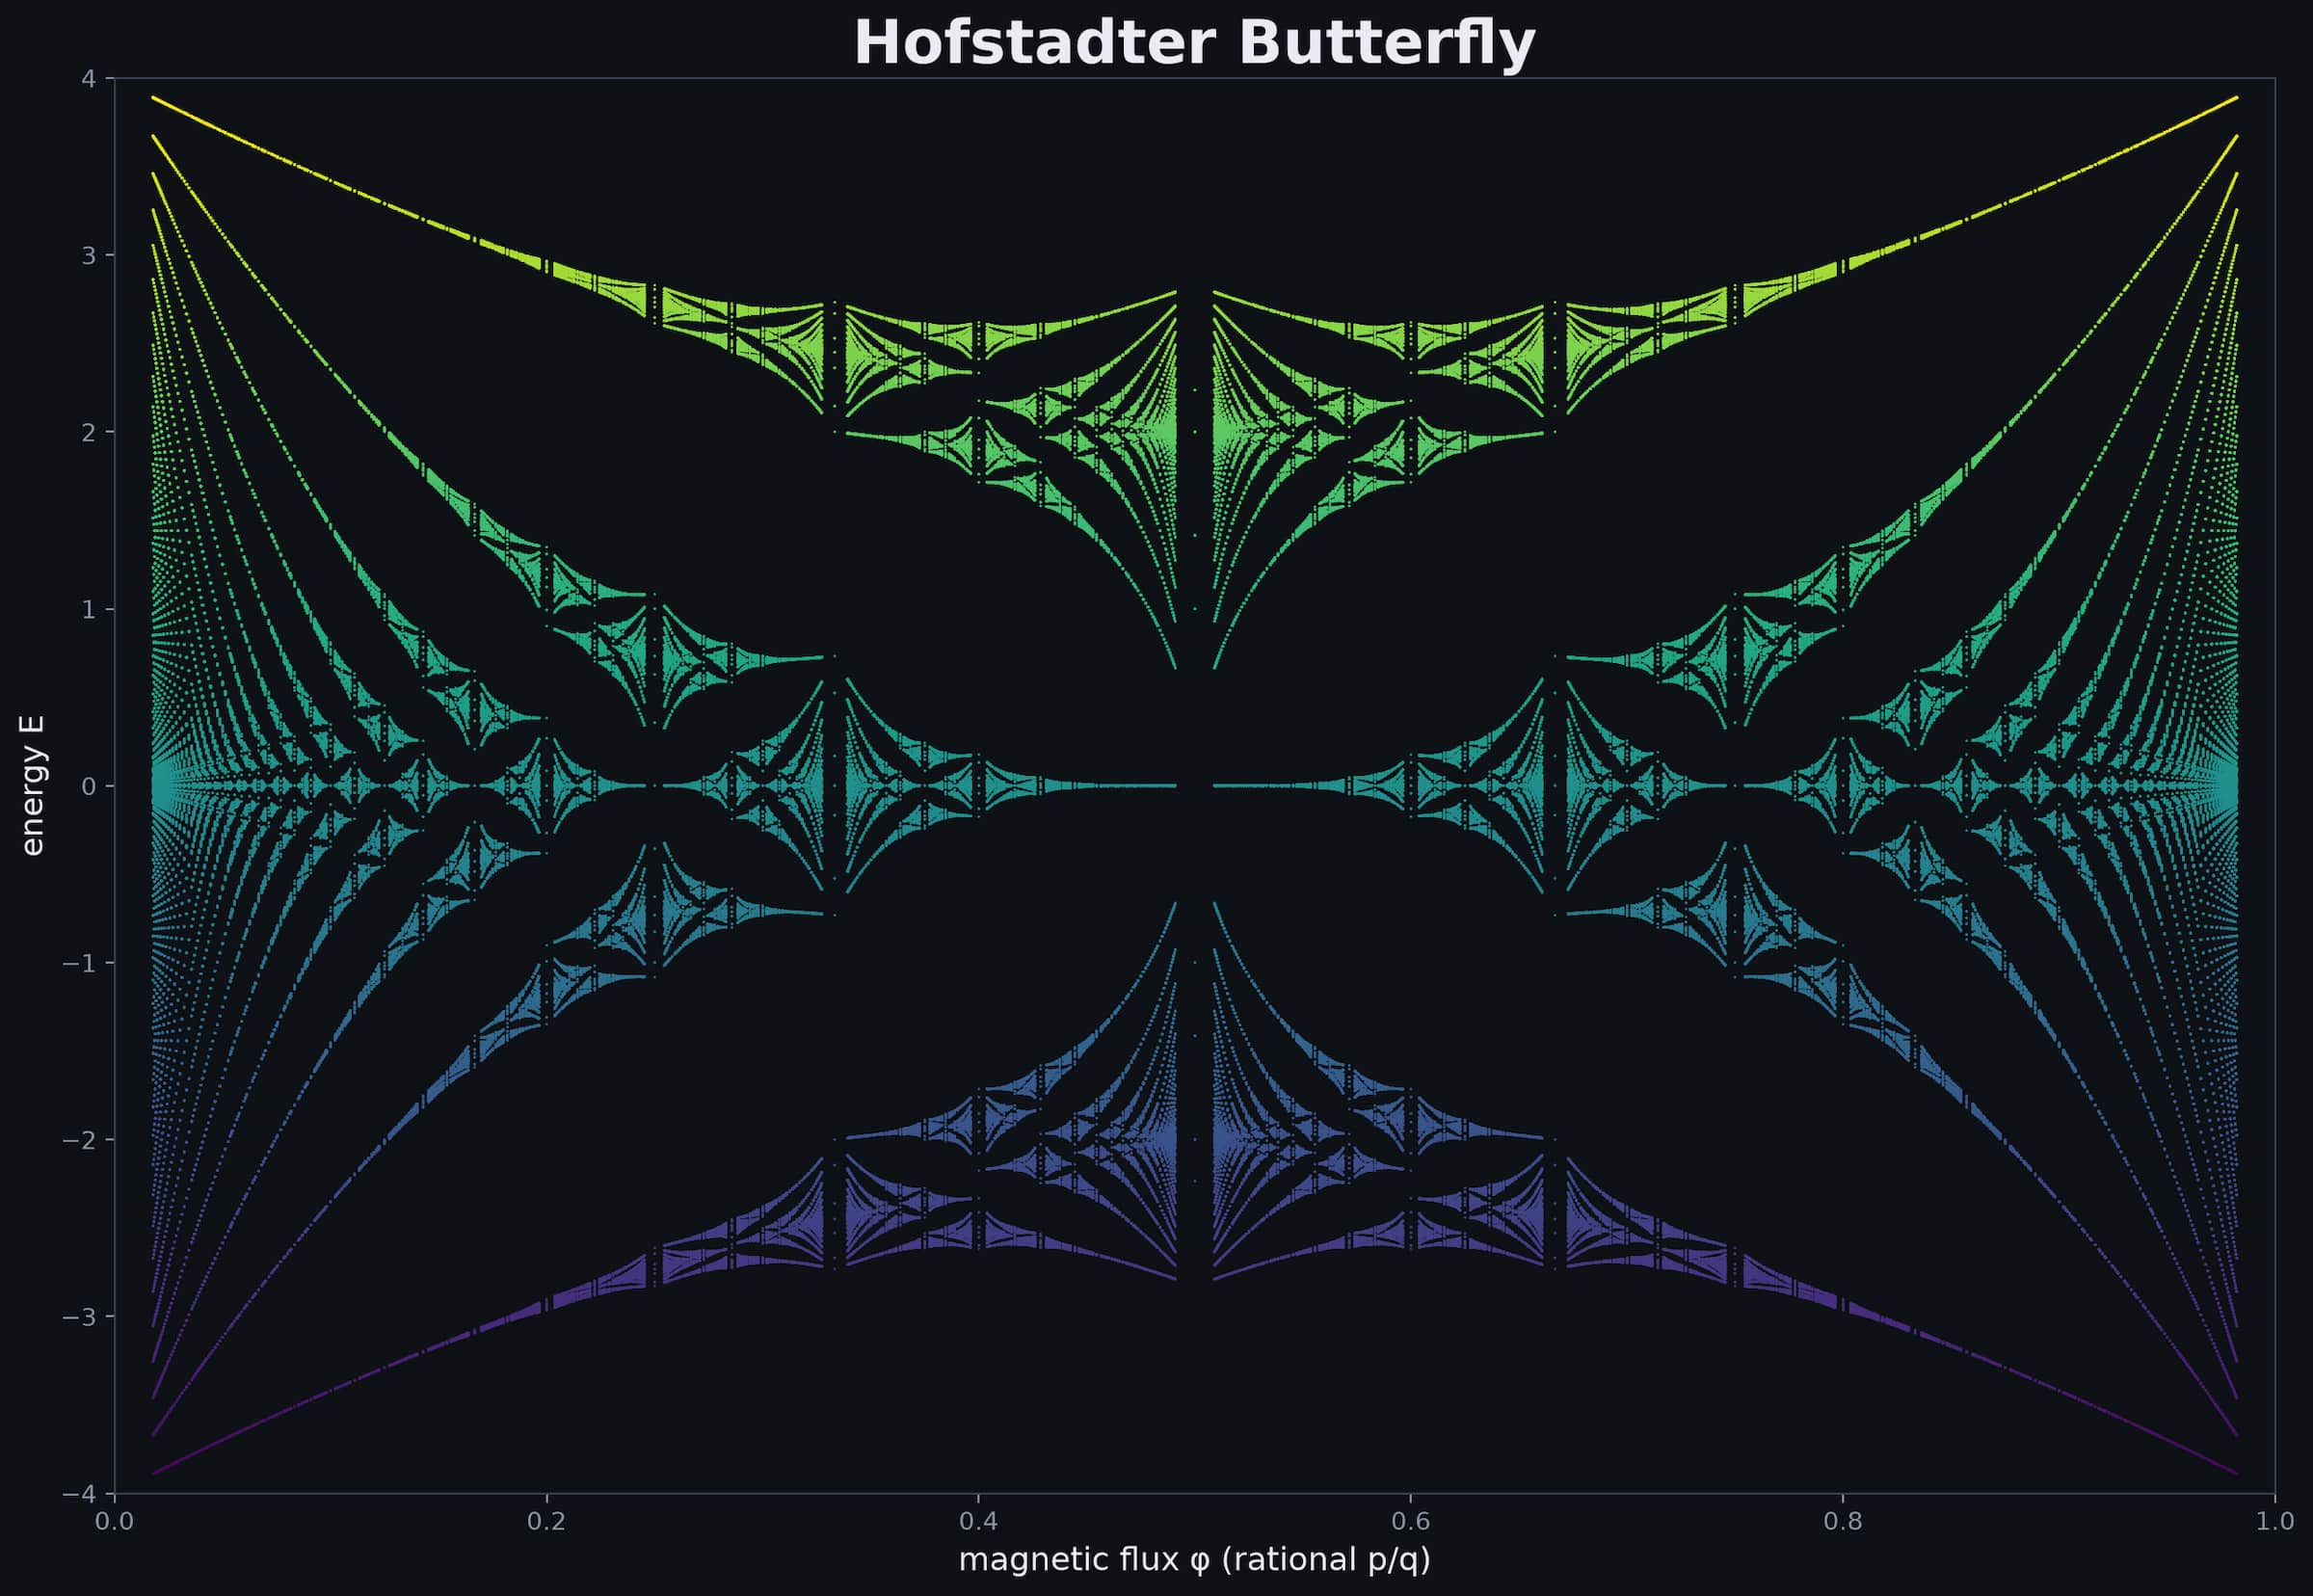
\includegraphics[width=0.90\linewidth]{graphs/hofstadter}
    \caption{Description of the figure. Replace \texttt{graphs/hofstadter} with
    your own file — any PNG, JPG or PDF in the project folder, without the
    extension.}
    \label{fig:single}
\end{figure}

As seen in \cref{fig:single}, the result shows ...

% ── TWO-PANEL SUBFIGURE (side by side) ──────────────────────
%    Two 0.48\linewidth panels plus \hfill fills the line.
\begin{figure}[htbp]
    \centering
    \begin{subfigure}[b]{0.48\linewidth}
        \centering
        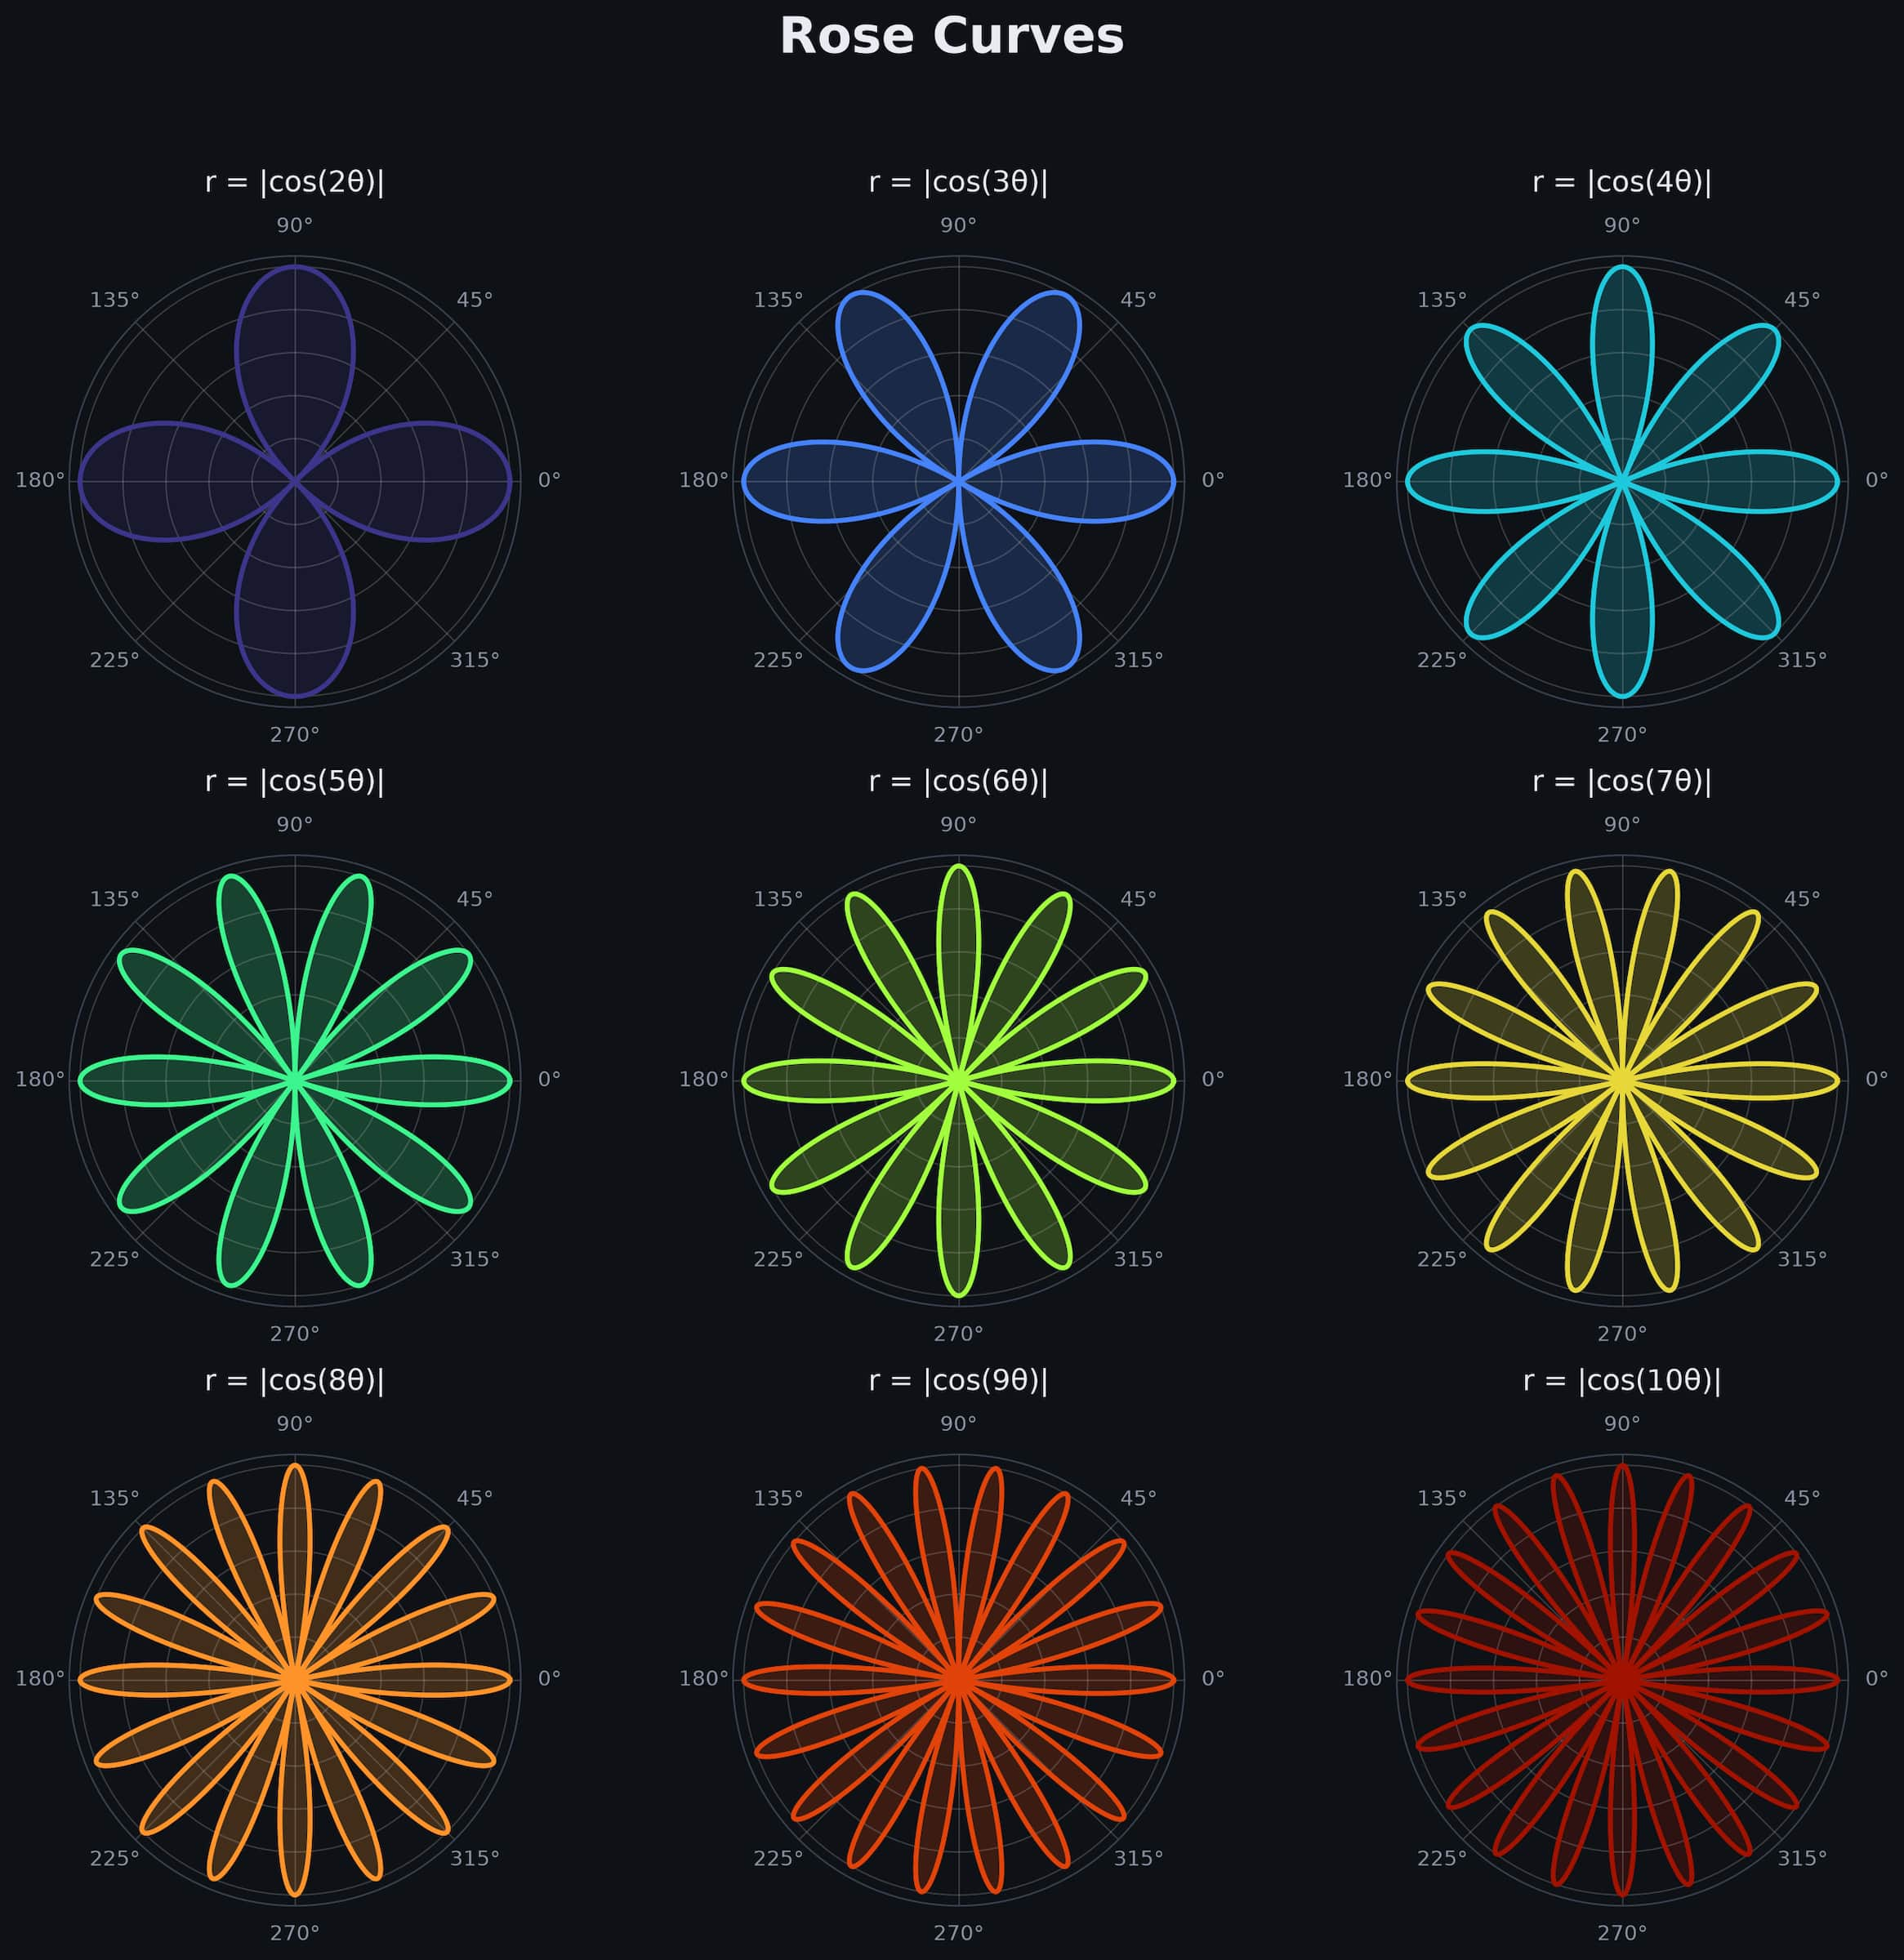
\includegraphics[width=\linewidth]{graphs/rose_curves}
        \caption{First configuration.}
        \label{fig:sub_a}
    \end{subfigure}
    \hfill
    \begin{subfigure}[b]{0.48\linewidth}
        \centering
        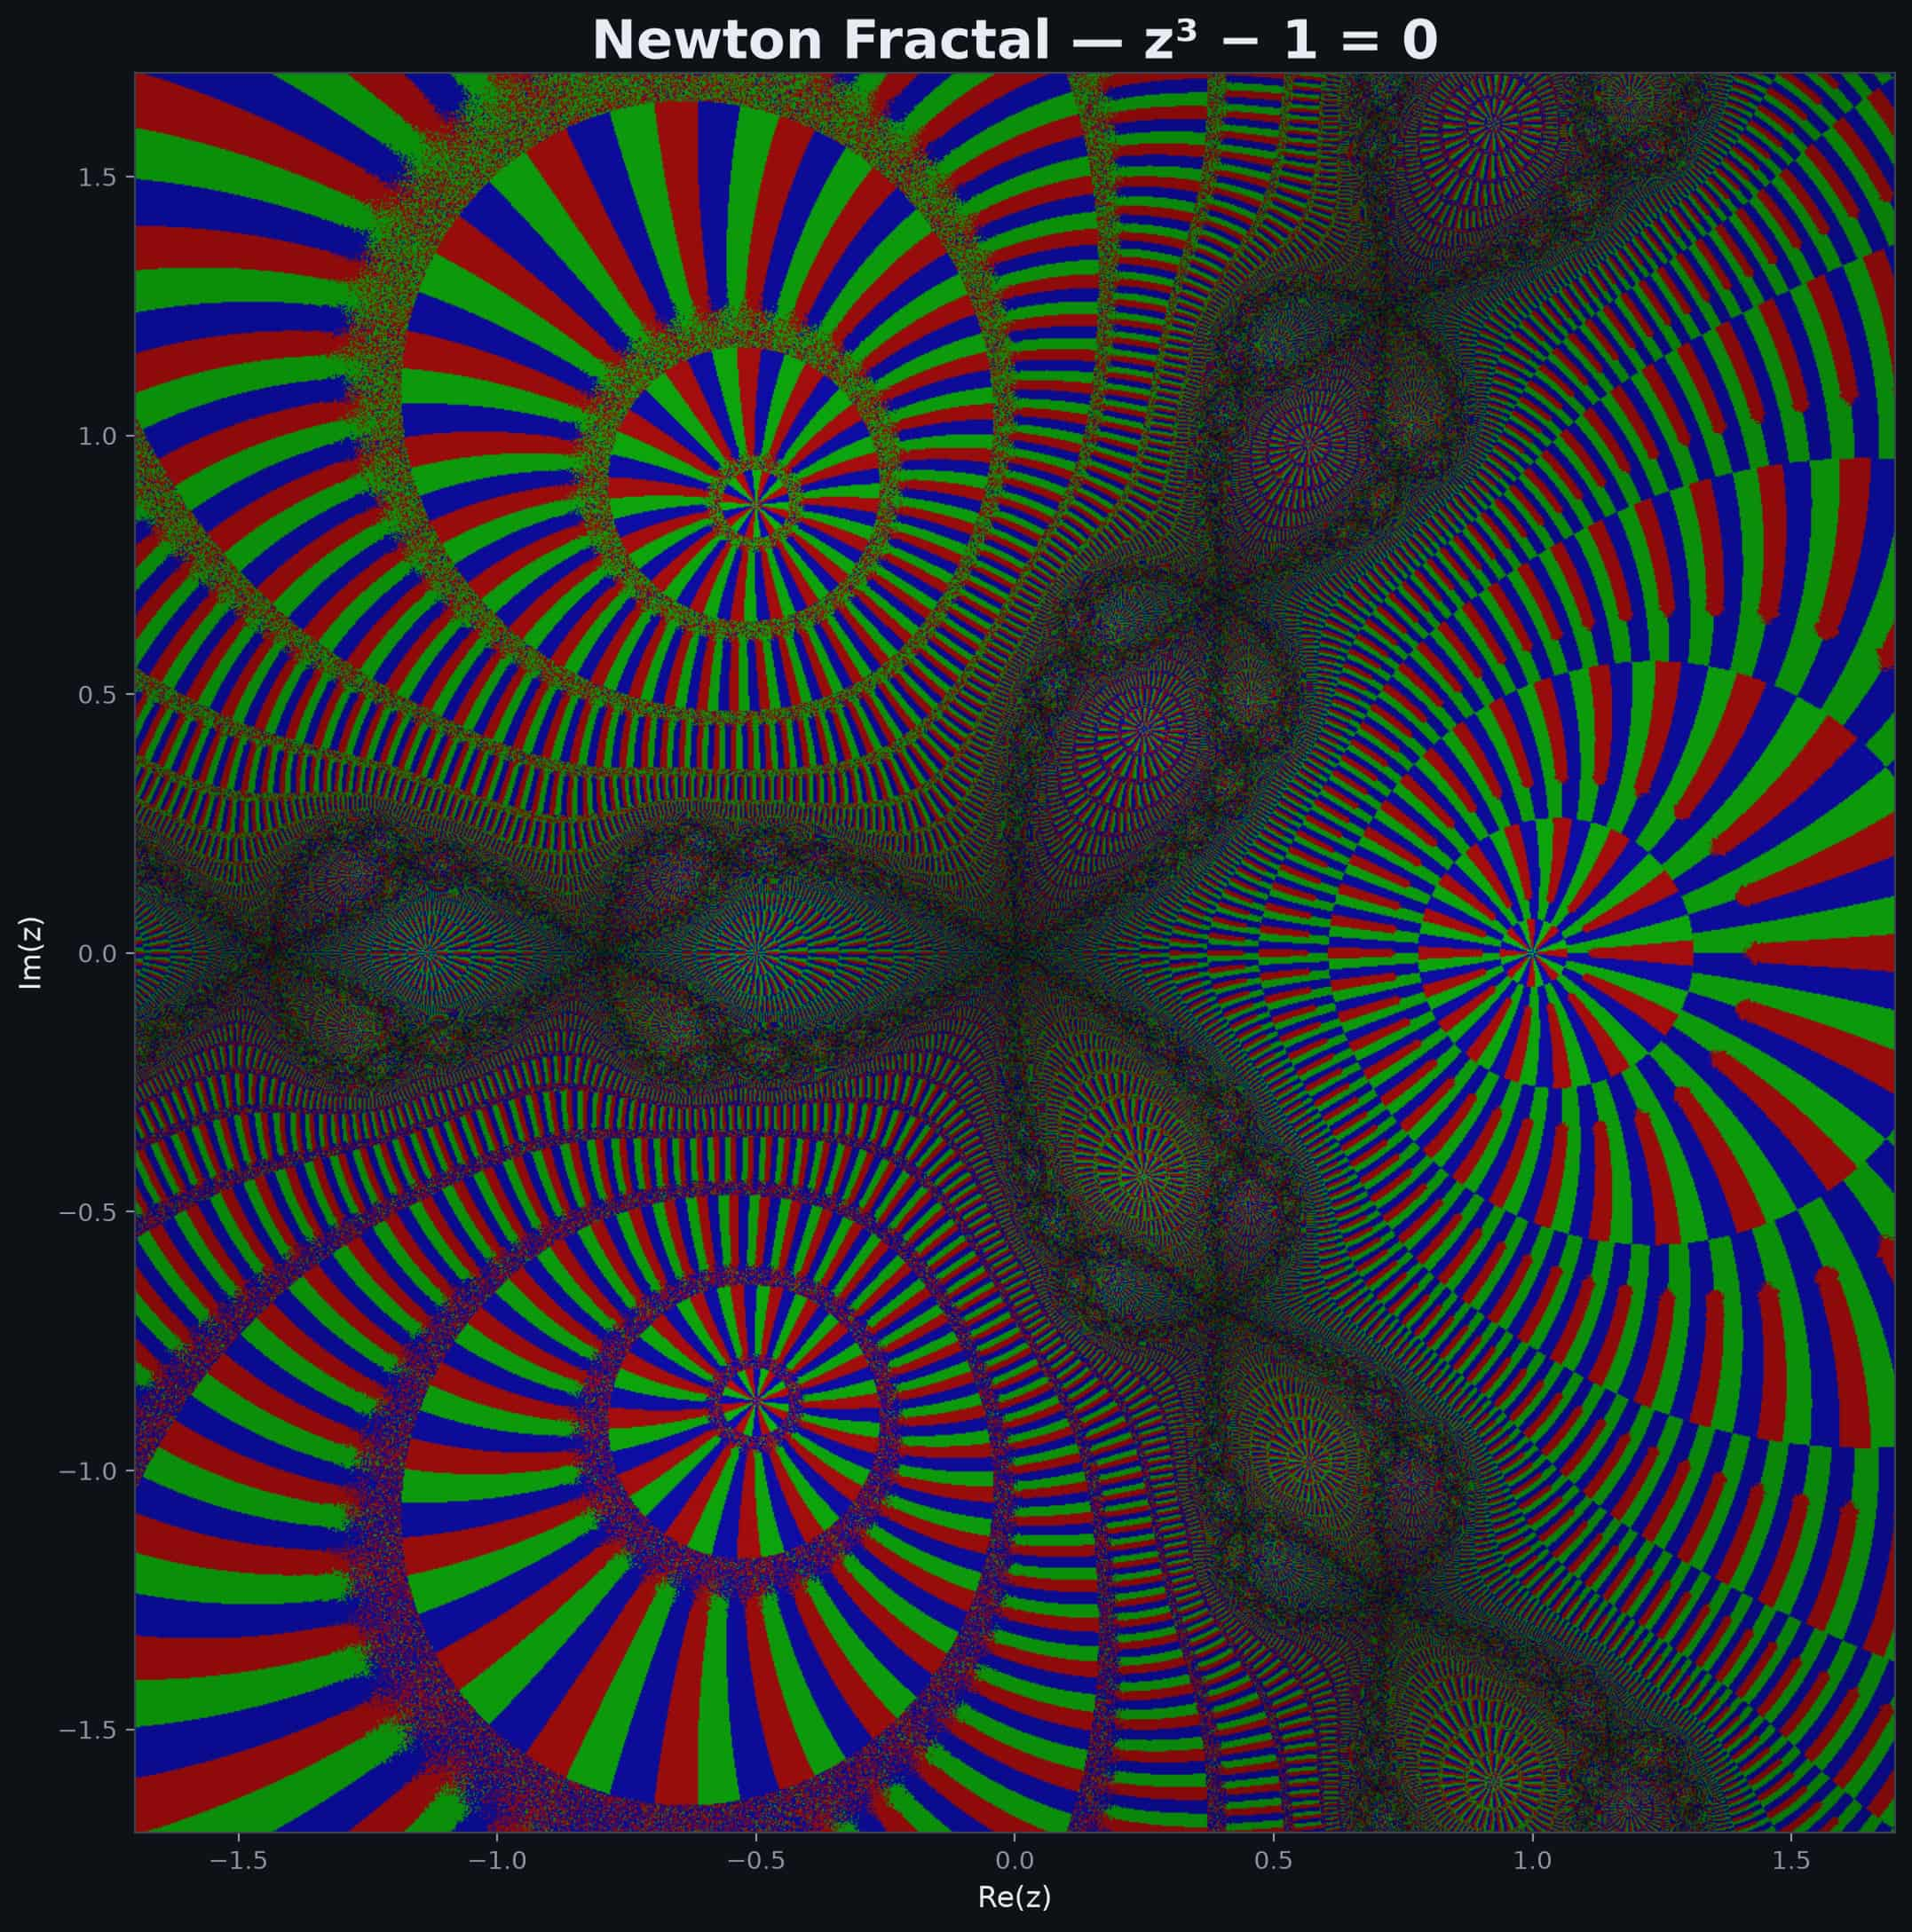
\includegraphics[width=\linewidth]{graphs/newton_fractal}
        \caption{Second configuration.}
        \label{fig:sub_b}
    \end{subfigure}
    \caption{Side-by-side comparison of (a) the first case and (b) the second
    case. Refer to one panel with \cref{fig:sub_a}, or to the whole figure
    with \cref{fig:sidebyside}.}
    \label{fig:sidebyside}
\end{figure}

% ── THREE-PANEL SUBFIGURE (stacked) ─────────────────────────
%    Same construction, one panel per line: leave a blank line
%    between the subfigures instead of \hfill.
\begin{figure}[htbp]
    \centering
    \begin{subfigure}[b]{0.40\linewidth}
        \centering
        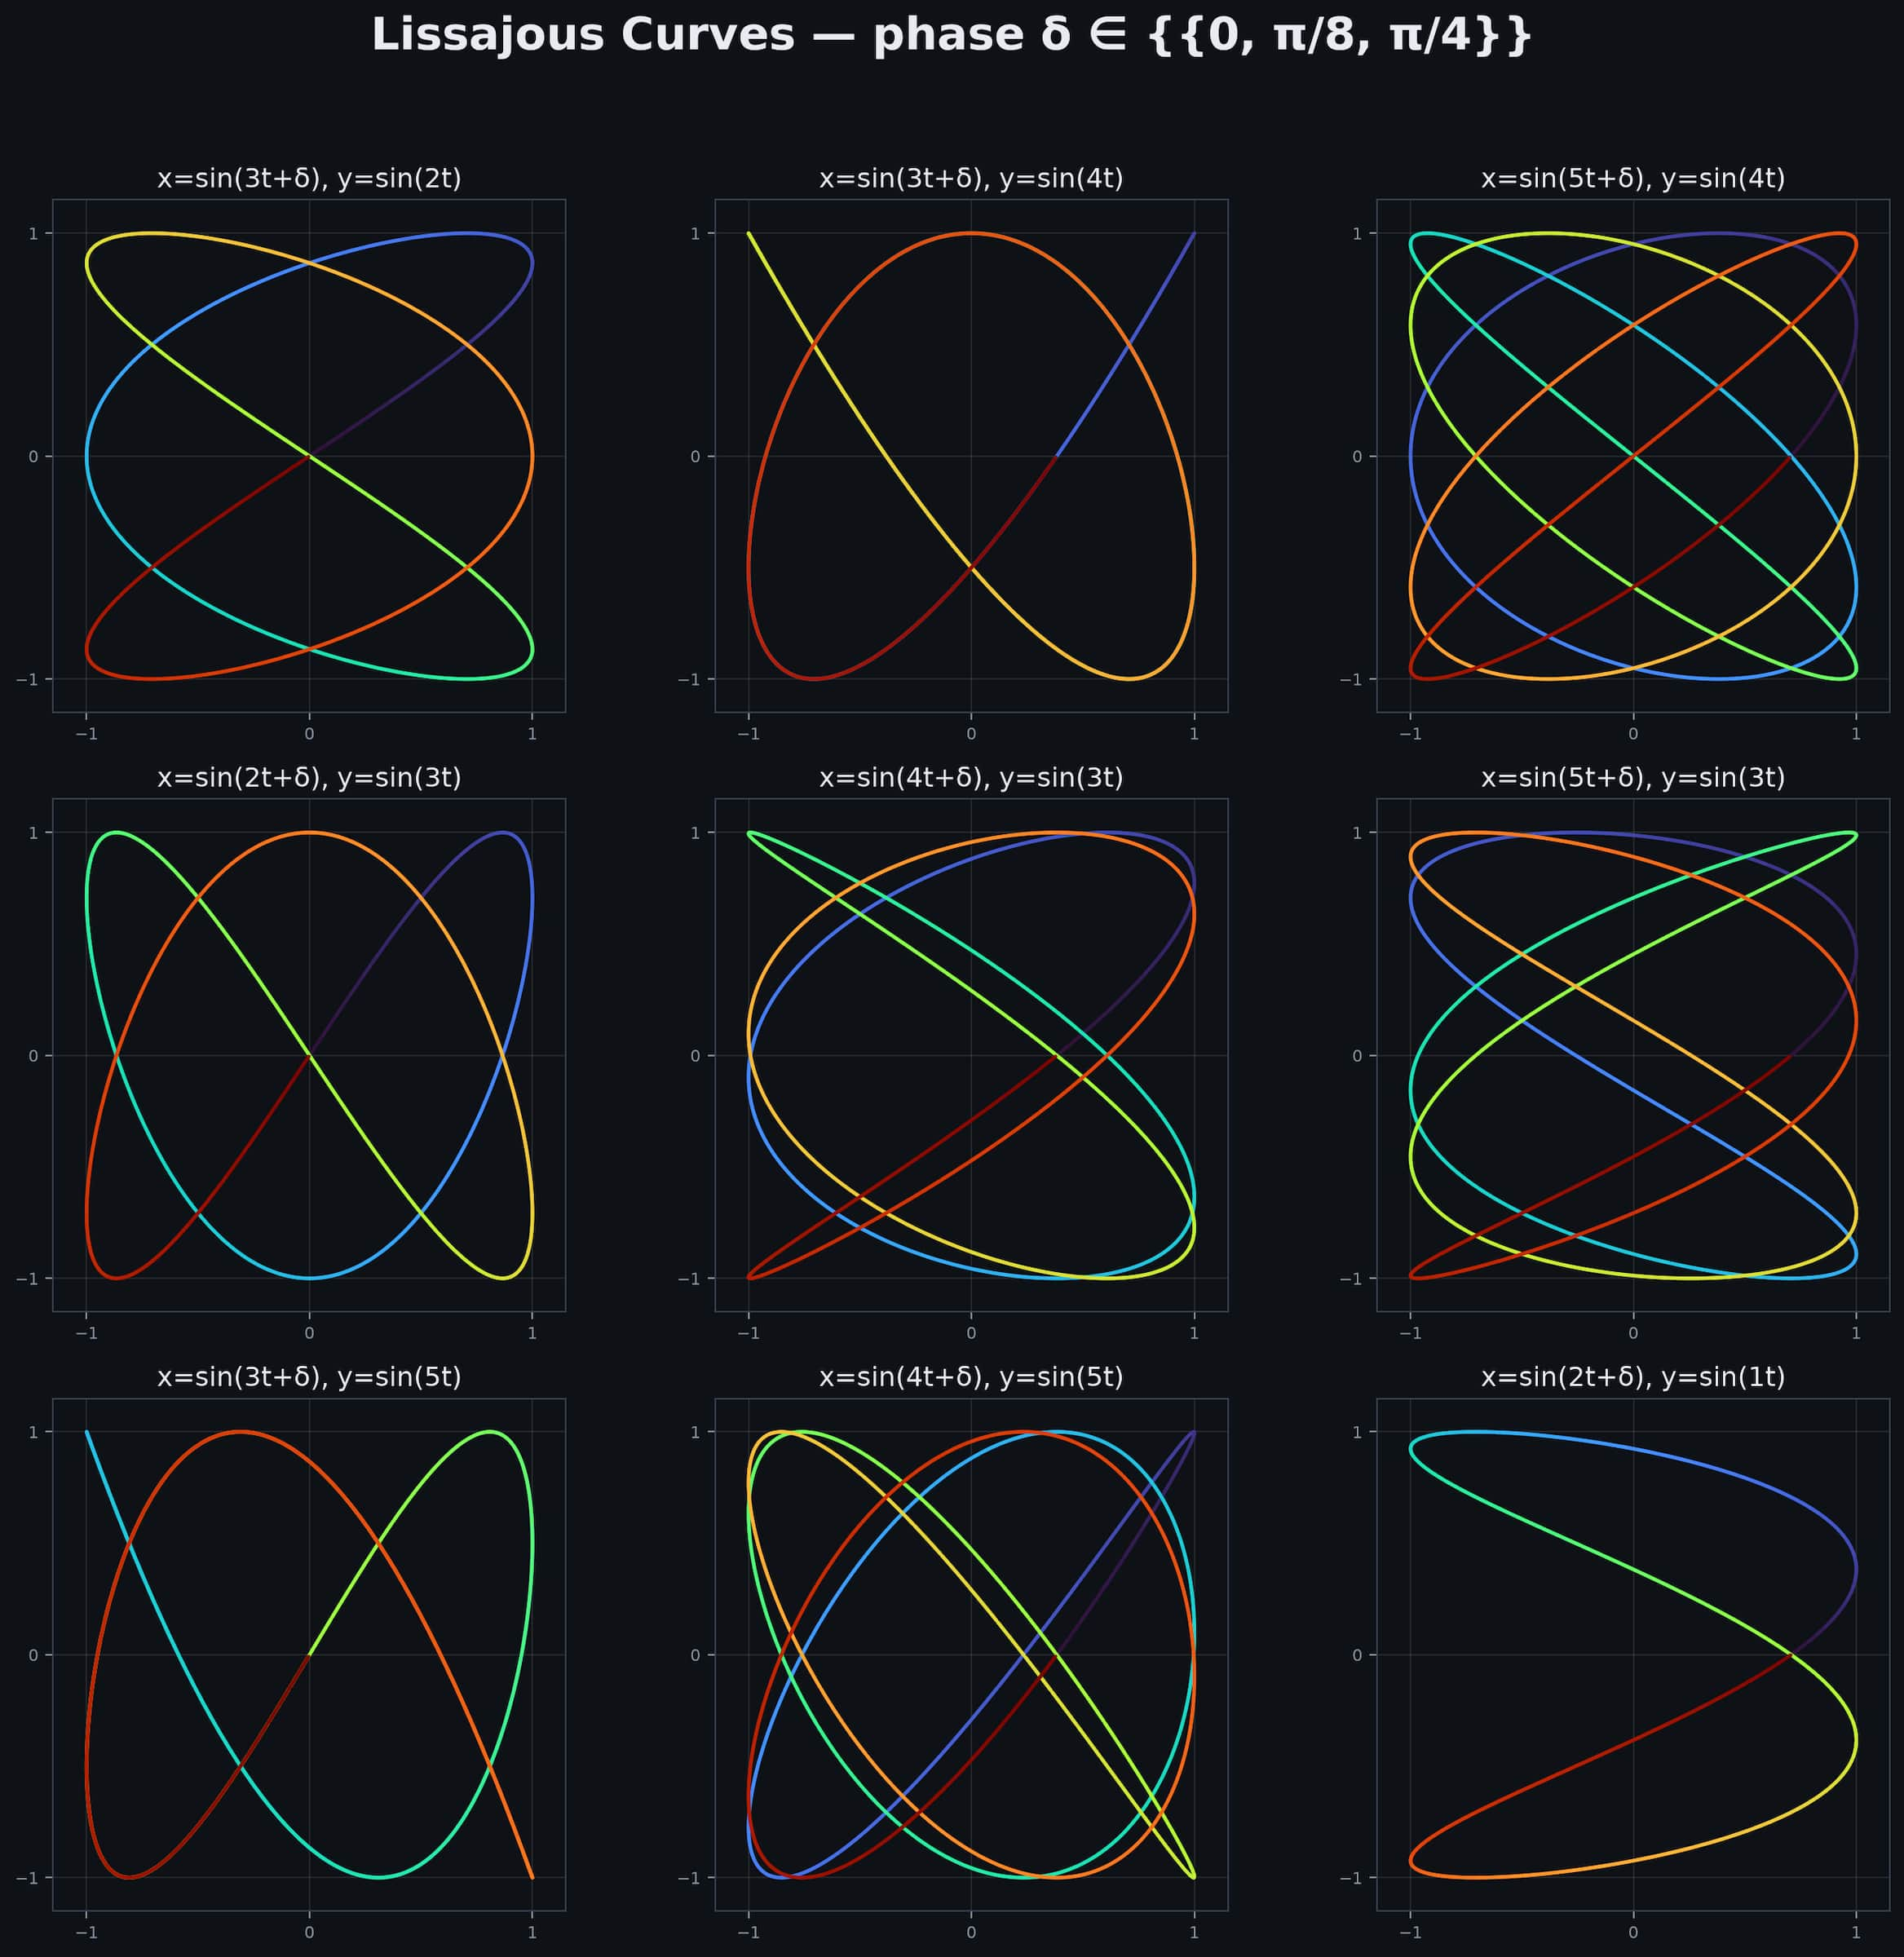
\includegraphics[width=\linewidth]{graphs/lissajous}
        \caption{}
        \label{fig:stacked_a}
    \end{subfigure}

    \begin{subfigure}[b]{0.40\linewidth}
        \centering
        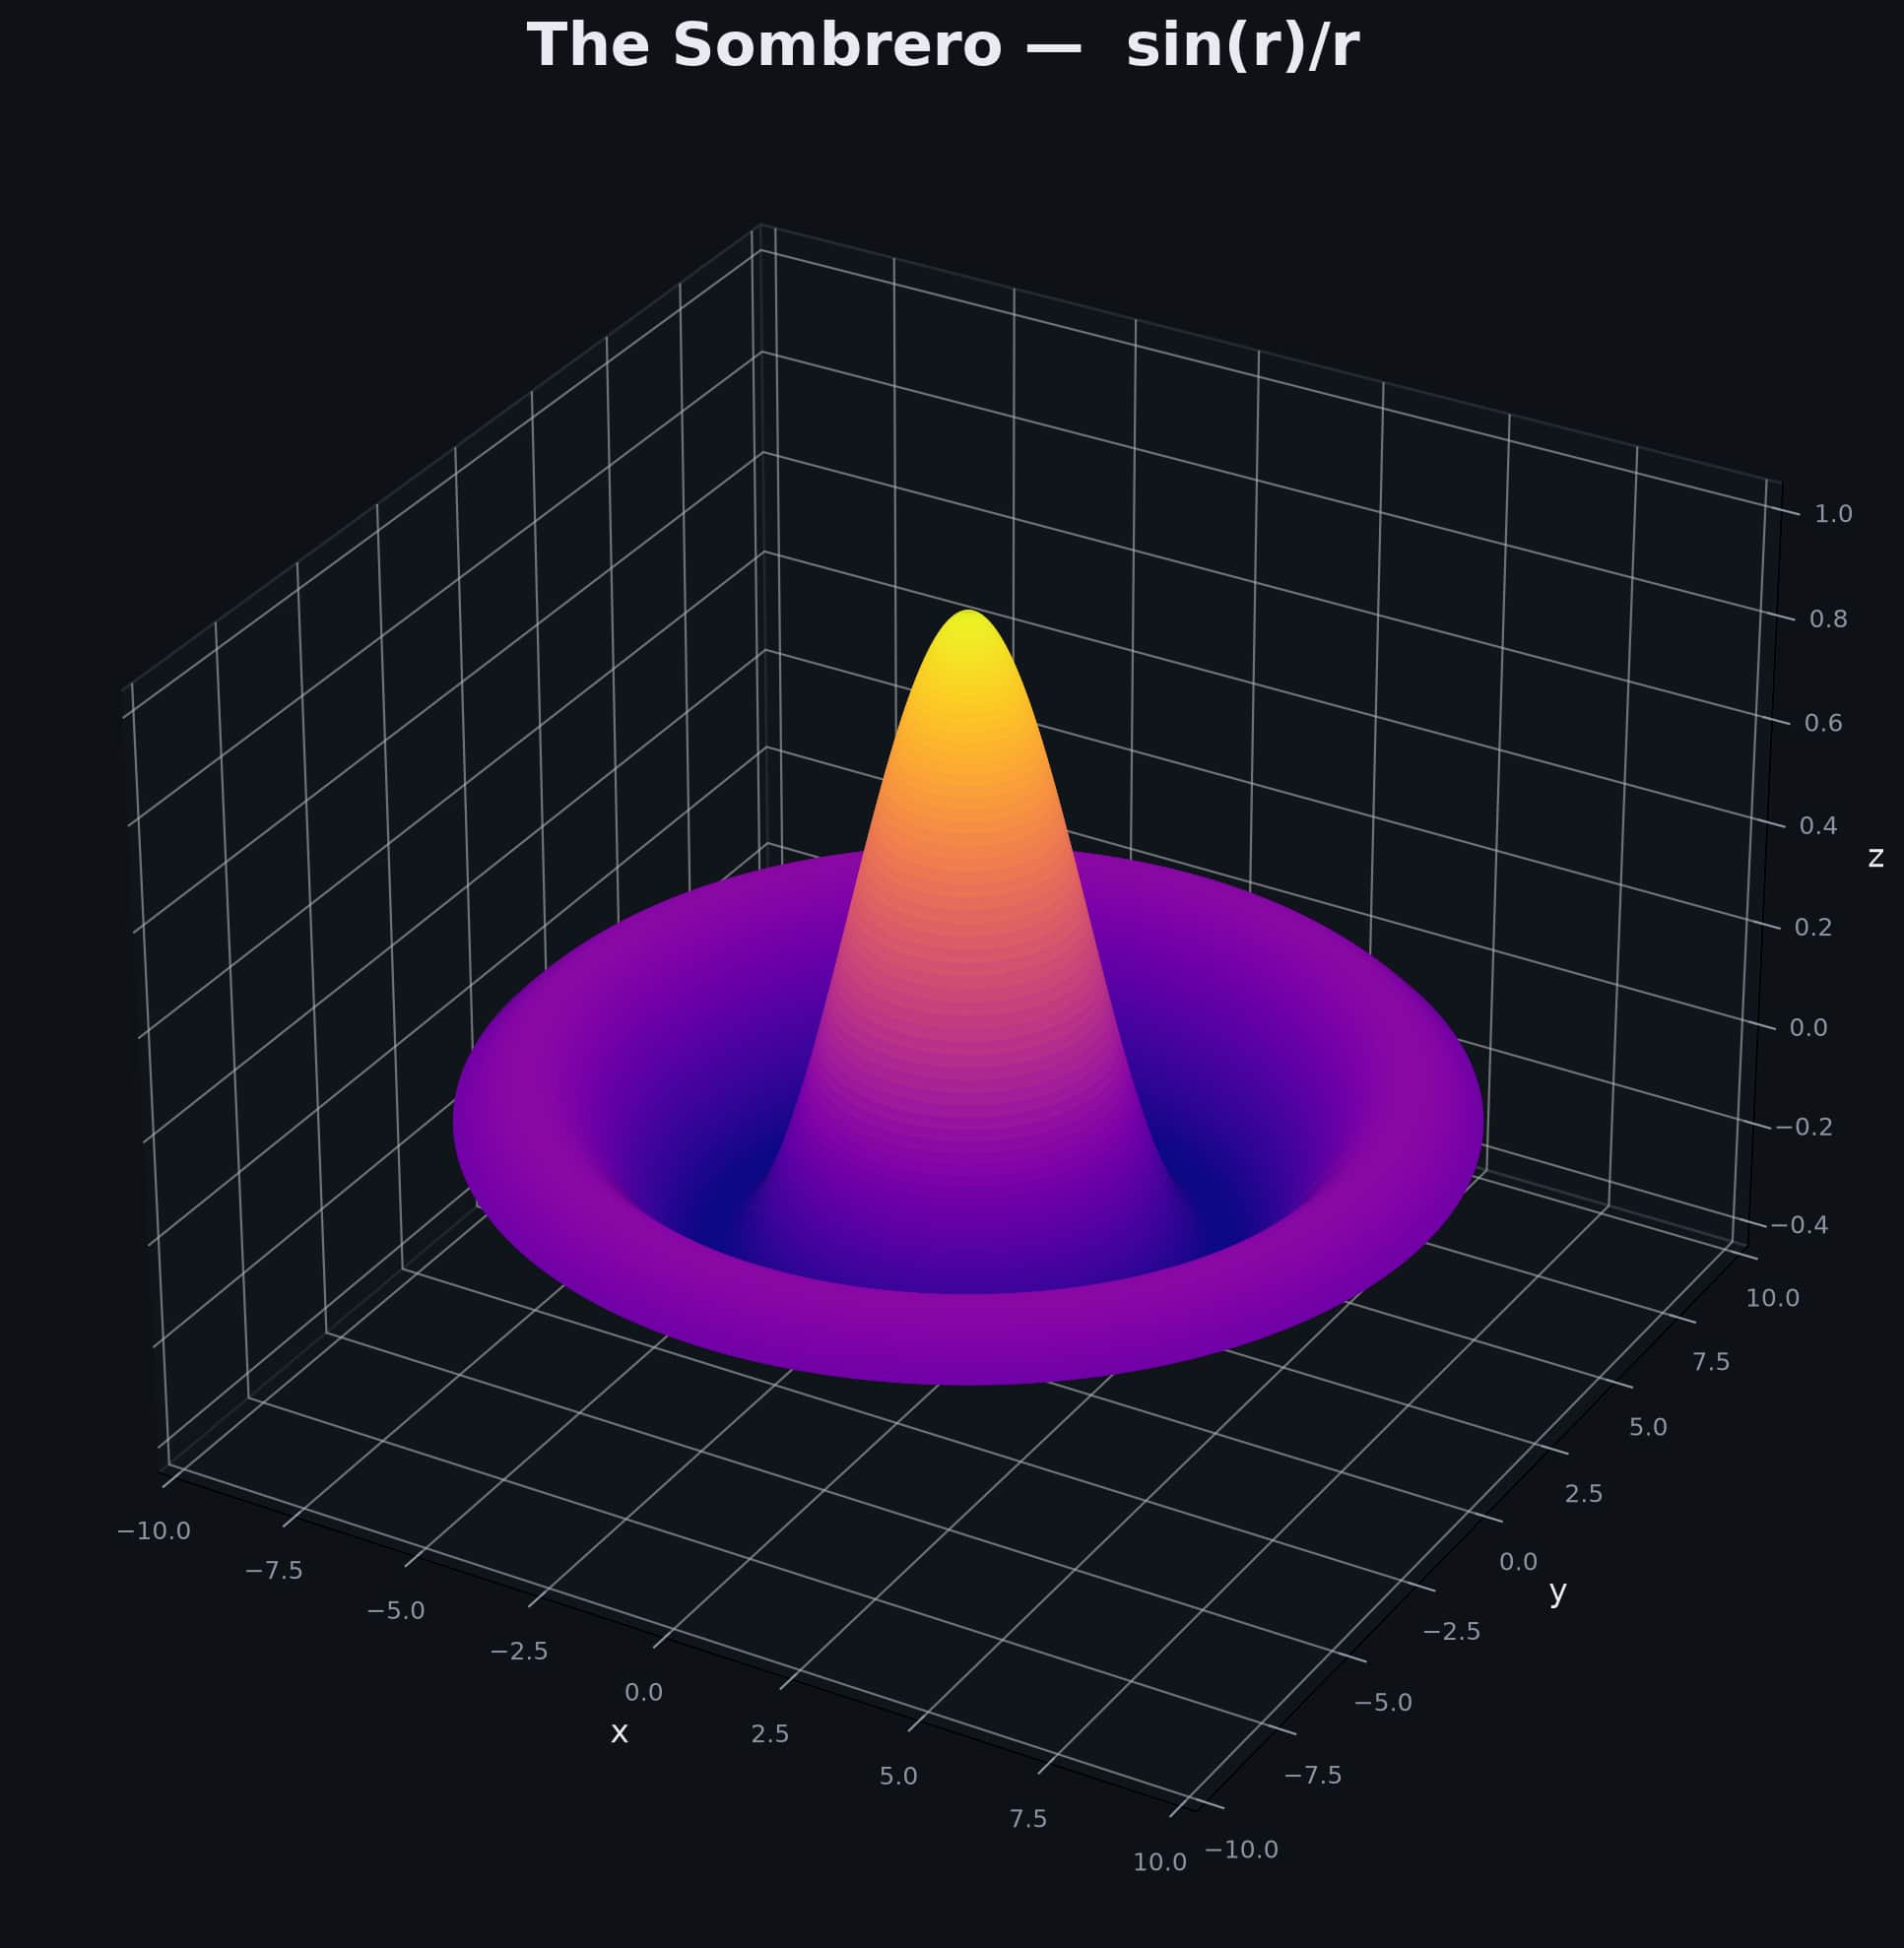
\includegraphics[width=\linewidth]{graphs/sombrero3d}
        \caption{}
        \label{fig:stacked_b}
    \end{subfigure}

    \begin{subfigure}[b]{0.40\linewidth}
        \centering
        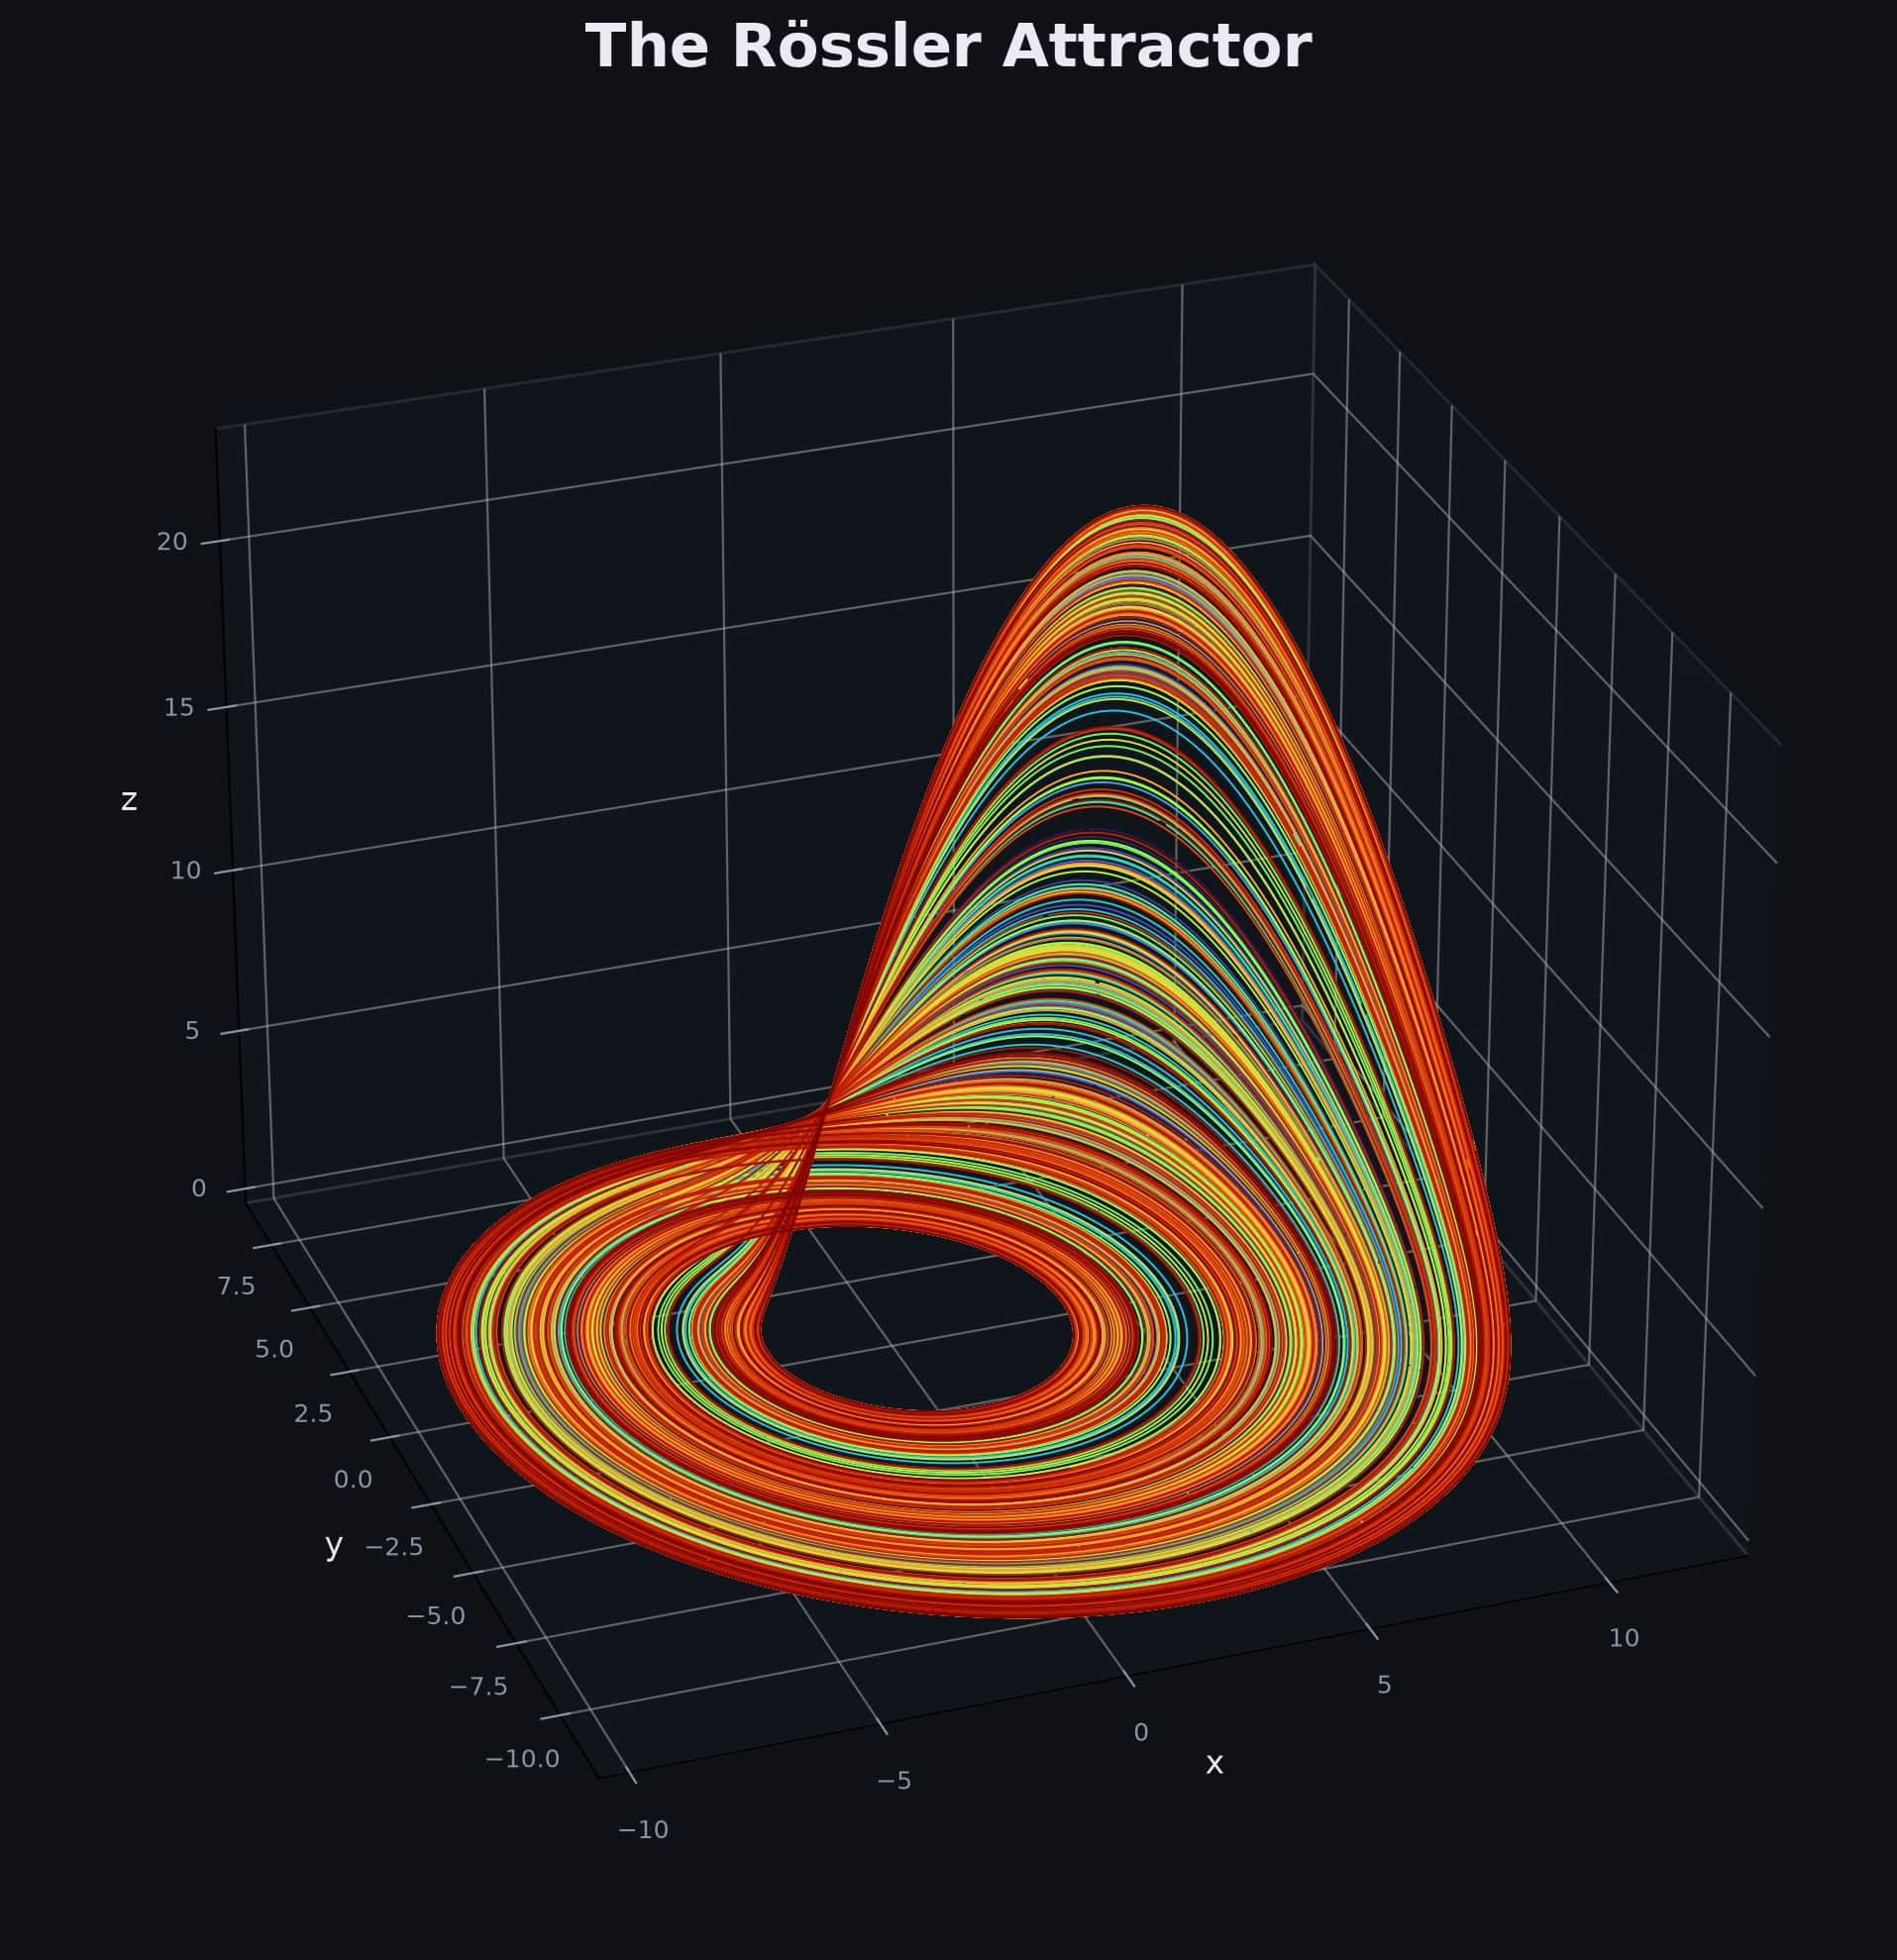
\includegraphics[width=\linewidth]{graphs/rossler}
        \caption{}
        \label{fig:stacked_c}
    \end{subfigure}
    \caption{Three results stacked vertically: (a) the first case, (b) the
    second, (c) the third. Empty \texttt{\textbackslash caption\{\}} calls
    leave the panels lettered but unlabelled, so the description can live in
    this caption instead.}
    \label{fig:stacked}
\end{figure}

From \cref{fig:stacked_a}, \cref{fig:stacked_b} and \cref{fig:stacked_c} the following can be noted: ...

% ── TABLE ───────────────────────────────────────────────────
\begin{table}[htbp]
    \centering
    \caption{Summary of numerical results for different parameter choices.}
    \label{tab:results}
    \begin{tabular}{|c|c|c|c|}
        \hline
        Parameter & Value 1 & Value 2 & Value 3 \\
        \hline
        $\alpha$  & 0.1     & 0.5     & 1.0     \\
        \hline
        $\beta$   & 2.34    & 1.87    & 0.99    \\
        \hline
        $f^*$     & 0.0012  & 0.0003  & 0.0000  \\
        \hline
    \end{tabular}
\end{table}

The results in \cref{tab:results} show that as $\alpha$ increases, the objective value $f^*$ decreases towards zero.

% ── WIDER TABLE (booktabs style, no vertical lines) ─────────
% Requires \usepackage{booktabs} in main.tex
\begin{table}[htbp]
    \centering
    \caption{Extended parameter sweep using booktabs formatting.}
    \label{tab:booktabs}
    \begin{tabular}{cccc}
        \toprule
        Iteration & $x_1$  & $x_2$  & $g(x_1, x_2)$ \\
        \midrule
        1         & 2.9989 & 0.4997 & 0.000000       \\
        2         & 3.0289 & 0.5078 & 0.000142       \\
        3         & 2.9590 & 0.4883 & 0.000323       \\
        4         & 3.0469 & 0.5114 & 0.000334       \\
        5         & 3.0078 & 0.5019 & 0.000010       \\
        \bottomrule
    \end{tabular}
\end{table}

% ── ALGORITHM FLOAT ─────────────────────────────────────────
%    Declared in main.tex with float.sty's \newfloat, because no
%    algorithm package ships in the browser engine's bundle.
\Cref{alg:newton} in Problem 3 describes the general structure. The specific update rule depends on the chosen method; see \cref{eq:update} for the greedy variant.

% ── FOOTNOTE ────────────────────────────────────────────────
The stopping criterion\footnote{A common alternative is to stop when the improvement between consecutive iterations falls below a tolerance $\varepsilon_{\text{tol}} = 10^{-6}$.} used here is a fixed budget of $T_{\max}$ iterations.

% ── Task b) ─────────────────────────────────────────────────
\subsection*{Task b)}
\phantomsection
\addcontentsline{toc}{subsection}{Task b)}

The implementation is carried out in Python. Key parameters are listed in \cref{tab:params}. The short excerpt in \cref{lst:p5_main} shows the core loop; for the full code see \cref{lst:p5_full} in the appendix.

\begin{table}[htbp]
    \centering
    \caption{Simulation / algorithm parameters used in Task b).}
    \label{tab:params}
    \begin{tabular}{|l|c|l|}
        \hline
        Parameter          & Value       & Description                    \\
        \hline
        $N$                & 100         & Population / swarm size        \\
        $T_{\max}$         & 1000        & Maximum iterations             \\
        $\Delta t$         & $10^{-3}$   & Time step                      \\
        $w$                & 0.7         & Inertia weight                 \\
        $c_1,\, c_2$       & 1.5,\ 1.5  & Cognitive / social constants   \\
        $\eta$             & 0.55        & Learning rate                  \\
        \hline
    \end{tabular}
\end{table}

% ── INLINE CODE LISTING (short excerpt) ─────────────────────
\begin{lstlisting}[language=Python, caption=Core optimisation loop (Problem 5), label=lst:p5_main]
import numpy as np

# --- parameters ---
N        = 100       # population size
T_max    = 1000      # iterations
x_min, x_max = -5.0, 5.0

def objective(x):
    x1, x2 = x
    return (x1**2 + x2 - 11)**2 + (x1 + x2**2 - 7)**2

# --- initialise ---
positions  = np.random.uniform(x_min, x_max, (N, 2))
velocities = np.zeros((N, 2))
best_pos   = positions[np.argmin([objective(p) for p in positions])]

# --- main loop ---
for t in range(T_max):
    for i in range(N):
        r1, r2 = np.random.rand(2)
        velocities[i] = (0.7 * velocities[i]
                         + 1.5 * r1 * (best_pos - positions[i]))
        positions[i] += velocities[i]
    scores   = np.array([objective(p) for p in positions])
    best_pos = positions[np.argmin(scores)]

print(f"Best x: {best_pos},  f = {objective(best_pos):.6f}")
\end{lstlisting}

The result obtained after running the code is $f^* \approx 0$ at $(x_1^*, x_2^*) \approx (3, 2)$, consistent with the known global minimum of the Himmelblau function.

\clearpage
